\documentclass{article}
\usepackage[utf8]{inputenc}
\usepackage[english]{babel}
\usepackage{biblatex}
\usepackage{graphicx}
\usepackage{listings}
\usepackage{fancyhdr}
\addbibresource{completedCILib.bib}

\begin{document}

% Fixing headers and footers
\pagestyle{fancy}
\fancyhf{}
\rhead{Valentin Hassinen}
\cfoot{\thepage}

\tableofcontents
\newpage
\section{Introduction}
Responsible code development is not a byproduct of good programmers, it is a paradigm of development in and of itself. 

The importance of this paradigm can be seen in the software issues of the past.
For example, the Therac-25, was a machine with software that had not been scrutinized, leading to catastrophic consequences. 
Similarly, the 2012 Knight Capital incident led to losses of millions of dollars because of issues stemming from integrating changes into an old system. 
The Y2K incident induced panic because widespread belief that internal clocks would cause system failures with the change to year 2000. 
Evidently, we need some standard procedures avoiding unreliable software so that we do not repeat the errors of the past.

Continuous integration (CI) is one such procedure. 
When developers make rapid changes, as they often do, they inadvertently introduce many issues to the stability and quality of the shared code base.
Consequently, we need to regulate this process of rapid changes and CI is that regulation procedure.
For example, CI, at the request of a change, includes the following events:
\begin{enumerate}
    \item It runs tests on the code base if the change is to occur.
    \item It controls the changes based on those test results.
\end{enumerate}

The purpose of this essay is to provide the reader with a thorough understanding of CI and its key components.

\section{The Tests}

Our intuition tells us that testing is about proving reliability, but is this really the case?
In favor, it seems evident that our purpose in testing is to build a program that works.
In contrast, because of the extensive amount of possible inputs it is implausible for testing to prove the reliability of a program. \cite{meyer_seven_2008}
Consequently, before developing tests, we have to ground our mindset and hope in reality, tests can only ever disprove reliability.

With our initial purpose dismissed, some negative reactions may arise.
For example, the temptation to dismiss testing may arise but this leads to us not detecting easy-to-catch bugs. 
Consequently, we may end up covering the bug in volumes of functionality, making these bugs into monsters.
Naturally, we have to avoid this, if we do not wish to go insane from the ensuing bug hunts.

\subsection{Manual Tests - The Depth of Mind}

A controversial claim is that humans were only needed in testing when computers were not advanced enough.
For example, we have short-attention spans, emotional issues and trouble remembering.
However, the mind through its flexibility has the ability to abstract and reason about code and this provides a degree of depth to analysis that computers has yet to match.
Consequently, a large portion of the CI process is designed to enable manual tests and if the CI process is to enable us, we have to produce an environment to counter-act these deficits. 

As a result, we have to distill what kind of environment works best with us.
For instance, there is the obvious manual approach that emphasizes the defect-hunting nature of testing.
However, if we focus our attention on defect-hunting, we will only be rewarded when we find a defect, this works against our short-attention span.
Moreover, the focus of defect-hunting is narrow, this ideology is only concerned with the present condition of the code. 
Evidently, this emphasis is not ideal, there are alternatives, for example, we can emphasize the problem-solving nature of testing.
If we emphasize the problem-solving nature, we will always be able to entertain ourselves with aspects of ideas in the code, the reward is continuous in the activity.
Furthermore, it emphasizes our ability to relate to abstractions of the code as it entertains future and past conditions of the code rather than being just concerned with the current defects.
Moreover, it makes a negative activity into a positive one, we are now working together to solve a problem rather than trying to find defects in the author's work.
As a result, we are leveraging our social life and, thus, preventing emotional issues.
In conclusion, there are good reasons to emphasize that our environment is to be characterized by problem-solving rather than defect-hunting.

\subsubsection{Tools to Aid Problem-Solving Discussions}
\begin{itemize}
    \item Code referencing
    \begin{itemize}
        \item Github
        \item Discord
        \item GitLab
    \end{itemize} 
    \item Response referencing 
    \begin{itemize}
        \item Github
        \item Discord
        \item GitLab
    \end{itemize} 
    \item Diagramming\cite{nicole_johnson_increasing_2021}
    \begin{itemize}
        \item Excalidraw 
        \item Microsoft Visuo
        \item LucidChart
    \end{itemize} 
    \item Data handling
    \begin{itemize}
        \item Excel 
        \item Google sheets
        \item Trello
    \end{itemize} 
\end{itemize}

\subsubsection{Behavioral Guidelines for Healthy Discussions}

To foster healthy discussion, we must aid the reviewer. 
This means we want to avoid power dynamics, if people are afraid to voice their opinions, we will miss a lot of feedback.
Thus, we want to punish behavior that prides itself on the code and refuses to accept feedback.

However, we also want to enforce behavior that favors the author.
This means we want to avoid negative feedback, feedback that does not focus on the code but rather on the person.
Consequently, we are required to punish behavior that ridicules code.

\subsubsection{The Problem-Solving Process}
\begin{itemize}
    \item The old code review process focuses on a line-by-line evaluation of code changes. \cite{cassee_silent_2020}

    \begin{itemize}

        \item Pros
        \begin{itemize}
            \item Methodical
            \item High coverage
            \item Simple Protocol 
        \end{itemize}

        \item Cons
        \begin{itemize}
            \item Time-consuming
            \item Uneventful
            \item Repetitive
            \item Not practical 
        \end{itemize}
    \end{itemize}

    \item The Modern Code Review focuses on quick exchanges of ideas in the code. \cite{sadowski_modern_2018}
    \begin{itemize}
        \item Pros
        \begin{itemize}
            \item Focus on the abstraction or the bigger picture
            \item Eventful
            \item Uniqueness, the individual can shape the procedure
        \end{itemize}

        \item Cons
        \begin{itemize}
            \item Low code coverage 
            \item Misses coding mistakes
        \end{itemize}
    \end{itemize}   
\end{itemize}

So, given these characterizations, which process is right for problem-solving?
In the old line-by-line evaluation, its repetitive and uneventful nature plays into the deficits of mind.
On the other hand, our ability to work with abstractions shines in the modern approach.
Naturally, the modern approach is best suited for manual reviews as is also representative of the current industry standard.\cite{sadowski_modern_2018}

\subsection{Automated Tests}

However, if testing is only manual, then we are not leveraging the full capacity of the modern computer. 
These computers provide breadth, memory, availability and focus that humans cannot match. 
This is where the old process of manual code review comes in. \cite{cassee_silent_2020}
This approach is not irrelevant, it is just not a suitable task for our brains, but the simple formula is perfect for our computers.
Thus, we can also capture the bugs that can only be found by the rigorous line-by-line evaluation of code. 

\subsubsection{The Smart Input Selection}

When comparing automatic to manual test, an essential ingredient is input.
When manually reviewing we can choose good input to try. 
However, even though this is true for manual tests as can be seen by the sources supporting manual testing. \cite{sadowski_modern_2018} 
How does this hold up when we try to be clever about future failures?

The research shows that our attempts to predict good input for automatic tests fare worse than random input. \cite{meyer_seven_2008}
Thus, research shows that we should leverage the power of a computer, we should randomize our tests and remove their dependency on authors.
However we must be flexible, in some cases we are only interested in a specific input-output relationship, then it is best to control the input.

\subsubsection{A Modular Approach}

A central problem of automated tests is that we cannot follow the computer crunching millions of numbers and, so, we must somehow pinpoint where the failure originated.
A solution to this problem is the modular approach, it focuses on breaking down our program into components that interact with each other.
Thus, our tests can leverage this program structure and report back in what component or in what integration of components the failure occurred.

\vspace{20pt}
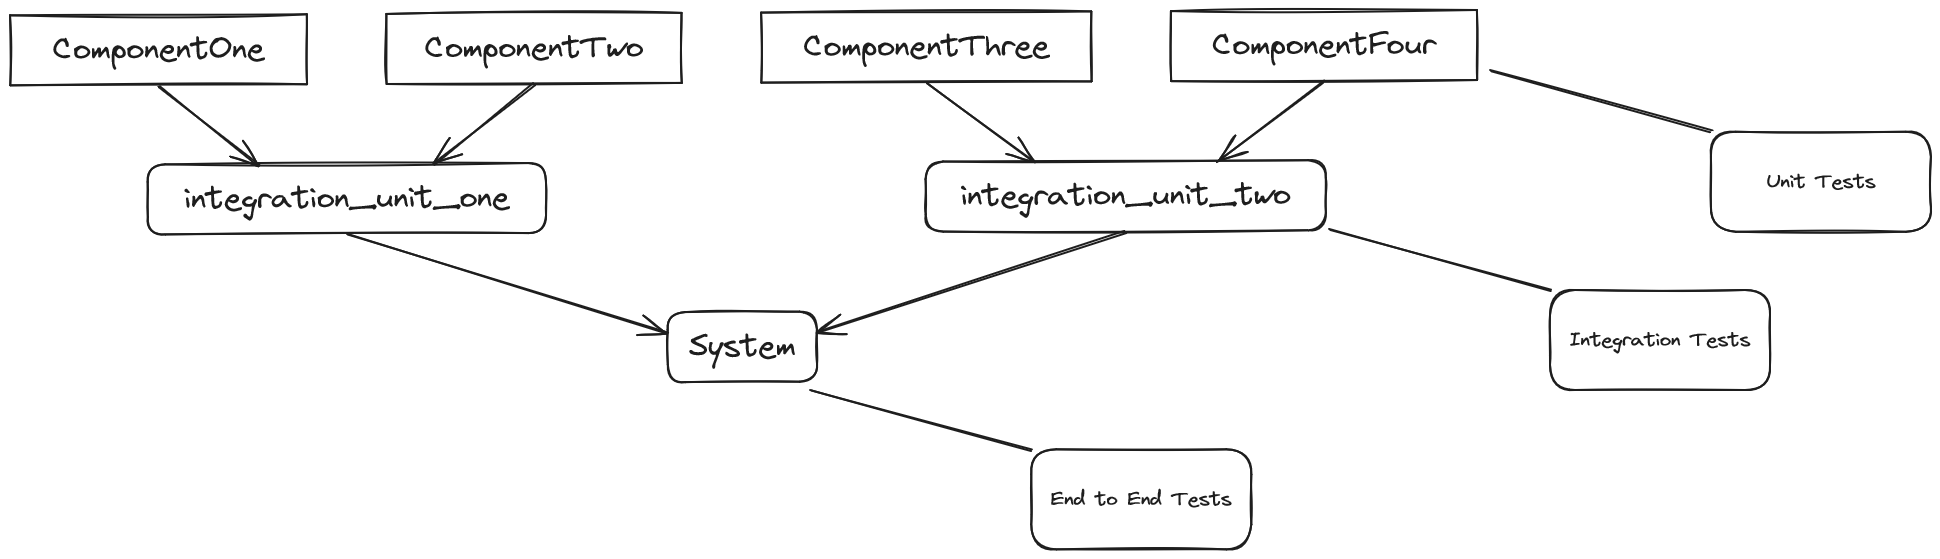
\includegraphics[width=\linewidth]{ModularizedTesting(1).png}

\newpage
\subsubsection{Automated Test Tools}

An important concept is that testing is not only a fail or pass process, the results can be continuous.
What CI does is produce an report from these automated tests.
Consequently, tools that track valuable information in the tests are essential in CI.

For example:

\begin{itemize}
    \item CPU Profiler
    \begin{itemize}
        \item Gprof (C)
        \item JProfiler (Java)
    \end{itemize}
    \item Coverage
    \begin{itemize}
        \item Gcov (C)
        \item Jacoco (Java) 
    \end{itemize}
    \item Memory Profiler
    \begin{itemize}
        \item Valgrind (C)
        \item JProfiler (Java)
    \end{itemize}
\end{itemize}

It is also important that we make the most out of our tools by making tests that have the specific tools in mind.
For example, for memory profiling we can replicate behavior that requires high memory allocation and, then, we can spot problematic areas.
Similarly, we can run tests characterized by a high volume of machine operations and then use the execution profiler to identify where most resources where used.


\subsection{The Manual and Automatic Synergy}

The full value of tests is only achieved once the two parts are brought together and that is the essence of CI. 
An important concept to note is that manual and automated tests can be run in different order to increase the benefit of the other.
We can then abuse these different orders depending on what we argue would have the greatest impact for the current change.

\subsubsection{Compacted Information - The Benefit to the Reviewer - Automation First}

Using automated tests, we can generate an insightful report from a line-by-line evaluation of the code.
This means that not only can reviewers delve into the ideas by reading the information given by the author. 
They can also analyze the results from various tests and leverage that to make an informed decision.
Thus, a more thorough analysis than just "this should work because the idea is sound" is achieved.

\subsubsection{Regression Tests - The Benefit to Automated Tests - Reviewer First}

The manual review sessions form an interesting feedback loop with automated tests. 
Any issue caught by a review can be made into a regression test.
A test that aptly named, prevents regresses, that is diving into issues that have been solved before.
Thus, we can use the human ability of depth to locate areas of a program that can be problematic and based on that develop more tests for those components.
Then, using the computers ability to remember we can ensure that this problem is spotted early in the future if it resurfaces.


\section{The Control}

Now given a thorough testing groundwork, we have finally reached the verdict, the point where a decision must be made. 

    How should we integrate the new change into the shared code base?

\subsection{Version Control Systems}

First, we need to mention how this integration decision is controlled and that in a modern environment through version control systems (VCS). 

This is essential for several reasons: 

\begin{itemize}
    \item Allow authors to work on their respective modules in parallel - Branches.

    \item Ability to do a rollback in case of older versions being more appropriate - Reverts.

    \item Effectively combine the works of different modules - Merges. 

    \item Track who changed code most recently to select reviewer - Blame. \cite{sadowski_modern_2018}


\end{itemize}

These are features that are often provided by a modern VCS. \cite{noauthor_version_2018}

\newpage
\subsection{The Feedback Control}

There is no one size fits all for what decision to make based on the analysis. 
On the other hand, we do have some software development standards and when deciding what standards we should look to the best practices.
However, we must also assess to what degree we can follow these best practices without sacrificing too much practicality.
Thus, a healthy discussion before the project must be met on the standards of the code base. 
Once this rule is set, the team should adhere to these rules when judging test results, preferably they are noted in the code base.
For example, an industry standard is to have a README file in the project, here we can list the project standards.

Some best practices are derived from this article \cite{noauthor_standards_nodate}:
\begin{itemize}
    \item Consistent code formatting and style:

    \begin{itemize}
        \item Which industry standard should we follow?
    \end{itemize}

    \item Code readability and documentation:

    \begin{itemize}
        \item Is the code too complex to analyze and debug?
        \item What is the average level of education and experience in the team? 
    \end{itemize}

\end{itemize}

\newpage
\section{A Worked Example: Our Java Calculator}

Now after having discussed the theory let's finish with a practical example, where we used CI for our product.

\subsection{The CI file}

To do the automated side of the CI process we use git actions. 
It runs the test automatically and it generates a report on the tests, this report contains test coverage and results.
This is a snippet from the file that builds and runs our tests using makefile commands:

\begin{lstlisting}    
    - name: Build Ast Tests
      run: make junit_build_ast
      working-directory: code
    
    - name: Build Parser Tests
      run: make junit_build_parser
      working-directory: code

    - name: Build System Tests
      run: make junit_build_system
      working-directory: code

    - name: Run tests
      run: make test_ci
      working-directory: code
\end{lstlisting}

As can be seen our tests are divided into ast, parser and system, the ast and parser are different modules.
The system tests are our end to end tests and in the ast and parser tests we have unit tests but also integration tests between components of those two larger modules.

The test environment we are using is junit

\subsection{A Photo of Test Runs}
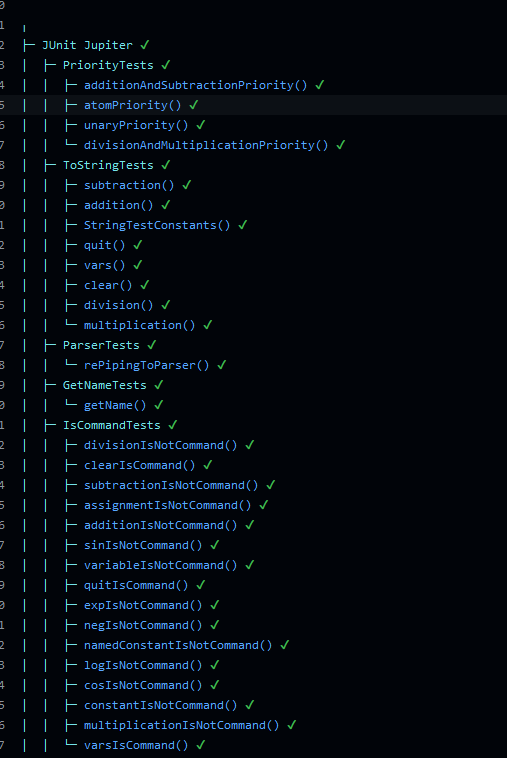
\includegraphics[width=\linewidth]{Screenshot 2023-11-29 161454.png}

\subsection{Protected Branch Control System}

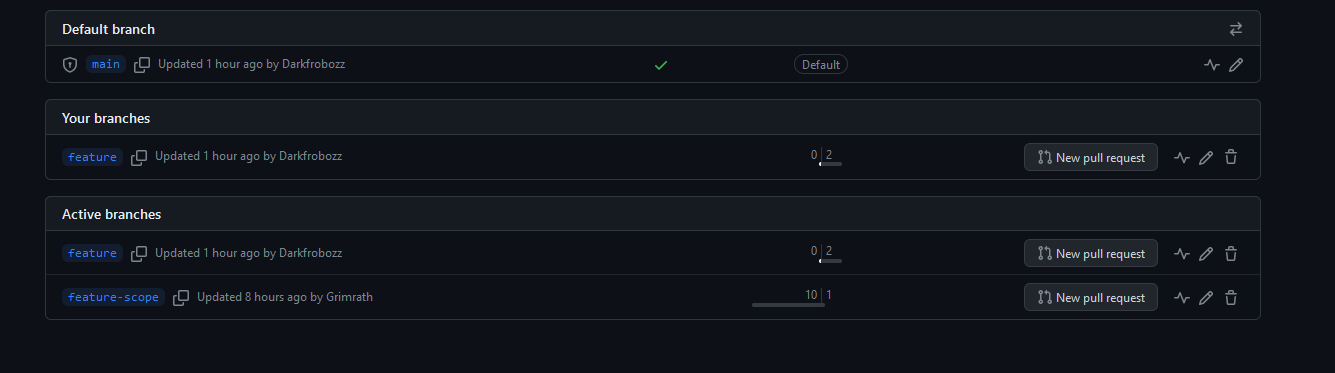
\includegraphics[width=\linewidth]{Screenshot 2023-11-29 161625.png}

Our main branch in this example is protected, so pushing is not allowed to main. 
To integrate an author's code, they must make a pull request and, then, the changed code must be reviewed and the tests for it must pass. 

\section{Conclusion}

This essay has highlighted the building blocks of CI, that is testing and control and how they integrate to form CI.
For example, It has explored what kind of testing is relevant in modern development and how control is decided.
In particular, the essay has focused on the exploration of manual reviews and how we can create the correct environment to foster this aspect of CI. 
This venture is undertaken because we need to discuss the human side of computer science more. \cite{senthil_behind_2023}
Moreover, it explored automated tests and how we can use smart input and modular design for maximum usefulness.
In addition, the result of analyzing these two components provided a framework for reasoning about how they can provide a better input to the other. 
The second step of the CI process was explored through introducing standard of code design and systems to control these changes.
Finally, a practical example of how several aspects of this process was applied in a real project was included to give the reader an illustrative example.
% Your content goes here
\newpage
\printbibliography
\end{document}